\chapter{State-of-the-art} \label{chap:State_of_the_art}

In the present chapter, a review of the current technologies related to the topic of this work will be done. Firstly, a review of different morphing wing technologies will be introduced. Secondly, a particular focus on the state-of-the-art of technology exploit in the current project will be presented.

\section{Morphing aircraft} \label{sec:Morphing_state}

  The interest in morphing of the aerodynamic surfaces has accompany aerospace history since the beginning. Since the first heavier-than-air flight in 1903, when the Wright Brothers designed and build a powered heavier-than-air aircraft that achieved the  first controlled and sustained flight. Their concept of aircraft did not provide importance to built-in stability but absolute control of the aircraft by the pilot. For this reason, they deliberatively designed their first aircraft with anhedral wing that make it dynamically unstable to perturbations in sideslip but more maneuverable in the lateral direction. In order to achieve roll control, they decided to incorporate a mechanism that would allow the wings to twist by pulling from cables, as it can be seen in Figure \ref{fig:Wright}. This was the first ever use of morphing of an aerodynamic surface for aircraft control. Since them, the necessity of enhanced performance and higher airspeed brought the requirement of stiffer wing structures to avoid aeroelastic instabilities.

  \begin{figure}[!htpb]
    \centering
    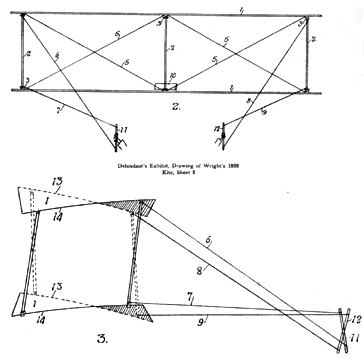
\includegraphics[width=0.6 \textwidth]{state-of-the-art/WrightBrothers1899Kite}
    \caption[Wright Brothers 1899 kite]{Wright 1899 kite: front and side views, with control sticks. Wing-warping is shown in lower view. \cite{Wright}}\label{fig:Wright}
  \end{figure}

  %Why to used them?
  On conventional aircraft, the need to modify the airflow around the airfoil at different flight conditions is achieve through discrete hinged mechanics such as flaps and ailerons. This mechanism perform well in a limited range around the design point while the outside this range, they have a negative influence in the aerodynamics. The necessary discontinuities that these elements produce on the surface, advance the boundary layer transition point from laminar to turbulent regime. Being able to modify the airflow without discontinuities on the surface would come along with notable reductions in parasite drag and therefore in fuel consumption.

  %Why now?
  New interest has raised in the recent years in aircraft morphing, mainly due to the appearance of new smart materials that allow more efficient mechanical design that do not necessarily incur in weight increments \cite{Lloyd2007}. Another reason that is pushing forward new aircraft morphing technologies is that missions today are in need of higher aircraft versatility to decrease operational costs in the commercial aviation field and aim to smaller and more distributed targets in the military field. For example, Airbus has recently patented a design of a downwardly foldable wing tip device applicable for a large passenger aircraft \cite{Boye2015}.

  %Different morphing projects - \cite{Barbarino}
  A general classification of different wing morphing concepts can be seen in Figure \ref{fig:morphingTypes}: planform modification through variation of sweep angle, span or chord; out-of-plane alteration involving twist, dihedral angle and spanwise bending, and airfoil adjustment achieved by modifications of the airfoil chamber and/or thickness. Under this classification, the morphing technology that is the focus of the work presented in this thesis is located under the out-of-plane branch and twist modification.

  \begin{figure}[!htpb]
    \centering
    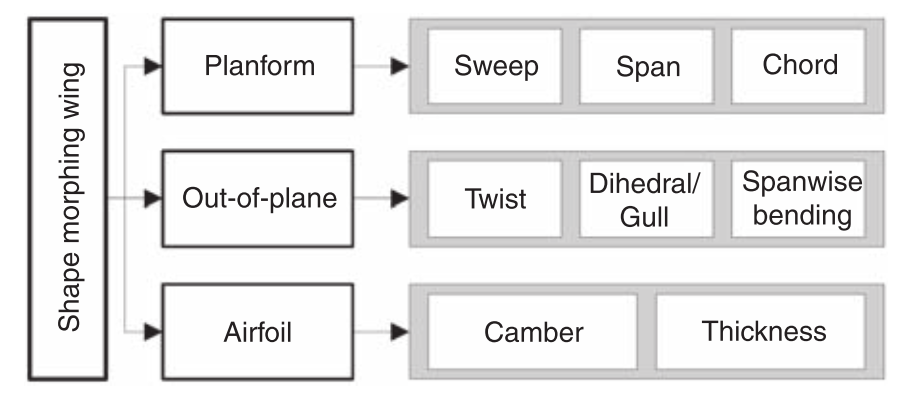
\includegraphics[width=0.8 \textwidth]{state-of-the-art/morphingTypes}
    \caption[Shape morphing wing classification]{Shape morphing wing classification. \cite{Barbarino2011}}\label{fig:morphingTypes}
  \end{figure}

  %NASA morphing proyect
  In the field of wing morphing through active aeroelastic concepts, the pioneer program of the Active Flexible Wing (AFW) was developed by Rockwell International in the 1980s \cite{Rockwell}. Under this program, a design of an aircraft where the wing aeroelastic twist was used to produce the required roll moments for control was generated. This enabled the aircraft to operate at dynamic pressures beyond those where convectional ailerons suffer from the appearance of reversal aeroelastic instabilities. Later, NASA continued with the AFW concept within their Active Aeroelastic Wing (AAW) project which used a modified F-18 fighter named X-53 to perform flight test and assess the viability of the proposed concept. The X-53 had its wings modified to reduce the torsional stiffness and had additional actuators added to operate the outboard leading-edge flaps separately from the inboard leading-edge surfaces \cite{NASA}. Rolling moment was obtained by aeroelastic twist of the wing using trailing-edge control surfaces and leading-edge flaps.

  %Here, many more references can be included by looking at Barbarino2011, maybe later... \section{Wing twist morphing}
  Following that initial attempts to deepen into the possibilities of wing twist morphing aircraft, many additional research literature can be found for other approaches. Many of those, consisted in modifying the wing properties by active means, i.e.: incorporating actuators that introduce energy into the system. However, wing twist morphing designs may also benefit from geometrically flexible structures if the aeroelastic energy from the airstream can be used to activate the shape changing mechanics. Such an approach may lead to passive morphings strategies that are always preferred since no additional energy is necessary to be introduced into the system and the usual weight penalties of morphing may be avoided if no additional actuators are needed. In such an approach the work presented in this thesis is embedded.

\clearpage
\section{Compliant chiral structure} \label{sec:chiral_state}
  % \citeauthor{Lakes1991}
  % \citeauthor{Bornengo2005}
  % \citeauthor{Prall1997}

  As mentioned in the introduction, it is the interest of this work to exploit the capabilities of materials with negative Poisson's ratio. Such materials expand laterally when stretched and contract laterally when compressed. In \cite{Lakes1991}, R. Lakes proposed that negative Poisson's ratios can result from a hexagonal microstructure of rotable nodes and bendable ligaments such as the one shown in Figure \ref{fig:chiral}. Such structures are known as non-centrosymmetric, hemitropic, or chiral; they are distinguishable from their mirror image; that is, they cannot be superposed onto them and they are not isotropic.

  \begin{figure}[!htpb]
    \centering
    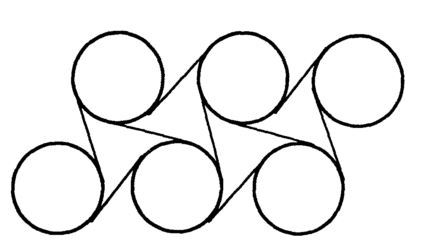
\includegraphics[width=0.6 \textwidth]{state-of-the-art/chiral}
    \caption[Chiral structure of rotable nodes and bendable ligaments]{Chiral (noncentrosymmetric) hexagonal microstructure of rotable nodes and bendable ligaments. Poisson's ratio is negative. \cite{Lakes1991}}\label{fig:chiral}
  \end{figure}

  In \cite{Prall1997}, experimental results showed that the a honeycomb chiral structure exhibited a Poisson's ratio of -1 for deformations in-plane. Indeed, this behavior was maintained over a significant range of strain, as shown in Figure \ref{fig:experimentalPoisson}, and therefore verifying that Poisson's ratio is independent upon the strain, in agreement with theory. 
  \begin{figure}[!htpb]
    \centering
    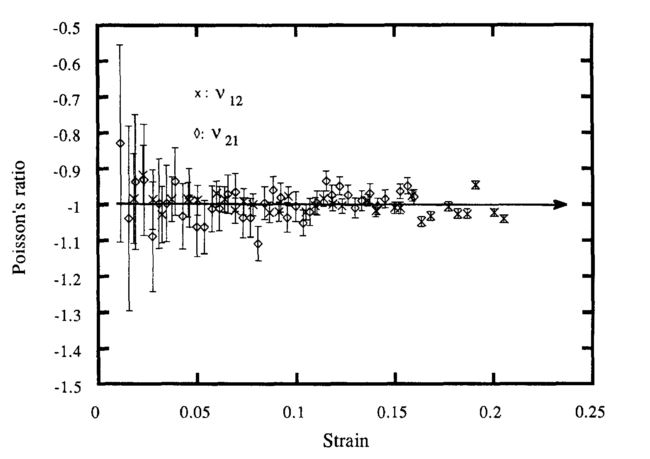
\includegraphics[width=0.8 \textwidth]{state-of-the-art/experimentalPoisson}
    \caption[Experimental Poisson's ratio $v$ as a function of axial compressive strain on a chiral honeycomb]{Experimental Poisson's ratio $\nu$ as a function of axial compressive strain on a chiral honeycomb. The error bars represent inaccuracies due to the measurement resolution. \cite{Prall1997}}\label{fig:experimentalPoisson}
  \end{figure}

  In \cite{Bettini2010} the properties of a chiral honeycomb are investigated, a manufacturing process using composite materials is proposed and the increase in the performance of using such materials is shown. Also, the experiments carried out allowed to characterize the possible failure modes of this structures and the nonlinear response when large displacements occur.

  Until that moment, most of the work was concentrated in studying the in-plane behavior of the chiral structures. Then, in \cite{Spadoni2005} the flatwise compression behavior of the chiral structures is investigated through FE modeling and simply analytical relations. This is the first consideration of buckling in a chiral structure in some way, in this case it was the out-of-plane buckling behavior based on the similar works presented in \cite{Zhang1992} and \cite{Gibson1999} for honeycomb structures. This research was extended by experimental studies in \cite{Scarpa2007} and an anelastic characterisation of the buckling phenomena is presented in \cite{Miller2010}. The use of controlled buckling for chiral honeycombs under a general macroscopic in-plane stress state was more recently investigated from a theoretical point of view in \cite{Haghpanah2014}. 

  %Buckling - Reference to work done by Gilles
  Within the research undertaken at the Laboratory for Composite Materials and Adaptive Structures (CMAS) of the ETH Z\"urich in the field of variable stiffness structures, a new design for the ligaments of the chiral structures has been proposed. This consists in the introduction of curvature into the chiral ligaments, as shown in Figure \ref{fig:ramstein-curved}. Each ligament posses double eccentricity which changes orientation at the centerline of it, in compliance with a equivalent connection with the cylinders located at the extremes. In \cite{Ramstein2016} experimental evaluation of the mechanical response of such structures is evaluated.

  This new design of the ligaments will provide additional tailorability over the buckling phenomena occurring on the lattice ligaments. This configuration is the one chosen for the chiral structure that is used in the concept presented in this work.

  \begin{figure}[!htpb]
    \centering
    \subfigure[Flat ligaments.]{\label{fig:ramstein-flat}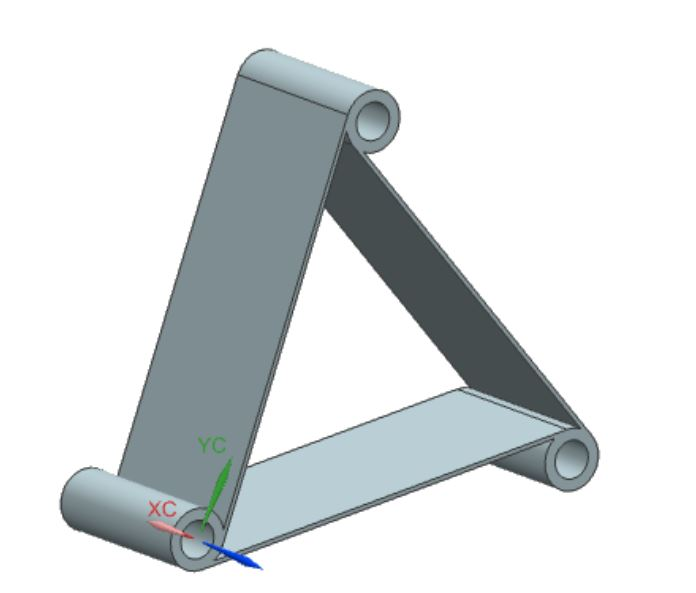
\includegraphics[width=0.4\textwidth]{state-of-the-art/flat-ligaments}} \qquad
    \subfigure[Curved ligaments.]{\label{fig:ramstein-curved}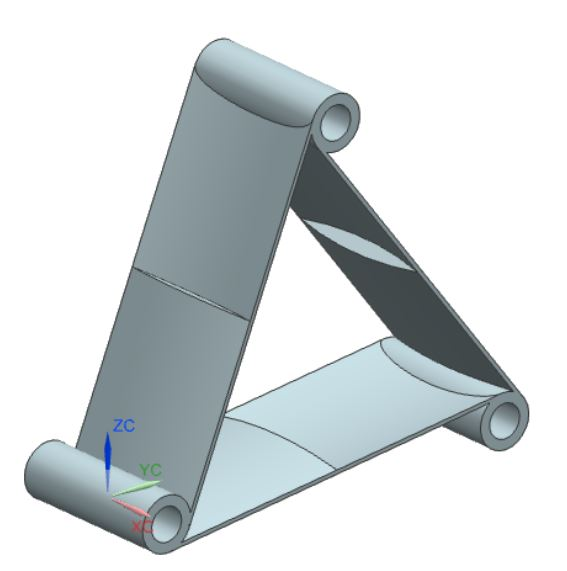
\includegraphics[width=0.35\textwidth]{state-of-the-art/curved-ligaments}}
    % \begin{subfigure}{0.5\textwidth}
    %   \centering
    %   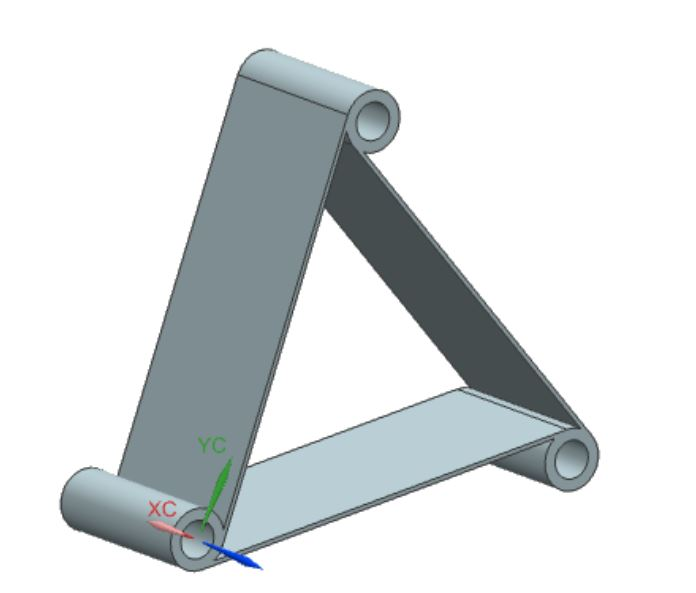
\includegraphics[width=0.4\linewidth]{state-of-the-art/flat-ligaments}
    %   \caption{Flat ligaments.}
    %   \label{fig:ramstein-flat}
    % \end{subfigure}%
    % \begin{subfigure}{0.5\textwidth}
    %   \centering
    %   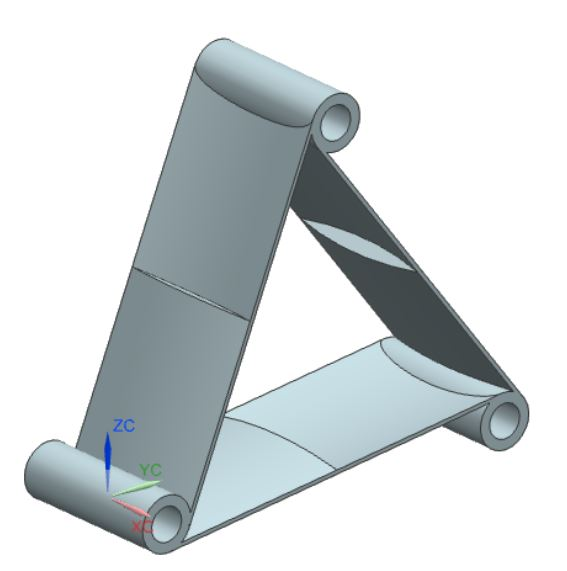
\includegraphics[width=0.4\linewidth]{state-of-the-art/curved-ligaments}
    %   \caption{Curved ligaments.}
    %   \label{fig:ramstein-curved}
    % \end{subfigure}
    \caption[Chiral cell elements showing different ligaments curvatures]{Chiral cell elements showing different ligaments curvatures. \cite{Ramstein2016}}
    \label{fig:ramstein}
  \end{figure}

\clearpage
\section{Chiral wing rib} \label{sec:wingRibChiral_state}

  Different approaches has been followed to exploit the particular characteristics of chiral structures on aerodynamic elements such as airfoils. In \cite{Bornengo2005} a truss-core configuration such as the one shown in Figure \ref{fig:truss-core-airfoil}(a) with chiral topology was utilized to design an airfoil for automotive competitions. The concept exploit the elastic deformation of the chiral lattice to modify the airfoil mean chamber line and thus modifying the pressure distribution as required for the current desired performance of the car. In \cite{Spadoni2007a}, a similar configuration was investigated by weakly coupled structural and CFD models, and the local and global deformations were characterized by consideration of the macroscopic chiral configuration. A prototype of the proposed design, as shown in Figure \ref{fig:truss-core-prototype}, was manufactured and tested in \cite{Spadoni2007b}. Results showed a remarkable tailoring of the chamber morphing performance by means of a limited number of parameters which define the core geometry. The dynamic properties of such chiral truss-core assemblies were investigated in \cite{Spadoni2006}.

  \begin{figure}[!htpb]
    \centering
    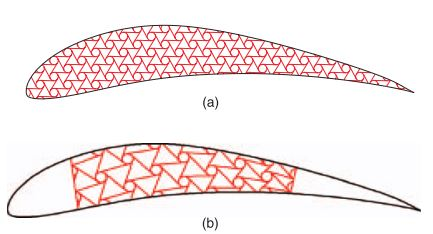
\includegraphics[width=0.7 \textwidth]{state-of-the-art/truss-core-airfoils}
    \caption[Investigated configurations for the truss-core of chiral topology]{Investigated configurations for the truss-core of chiral topology. \cite{Spadoni2007a}}\label{fig:truss-core-airfoil}
  \end{figure}

  \begin{figure}[!htpb]
    \centering
    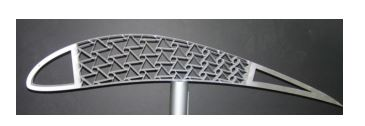
\includegraphics[width=0.8 \textwidth]{state-of-the-art/truss-core-prototype}
    \caption[Manufactured prototype of a truss-core airfoil with chiral topology]{Manufactured prototype of a truss-core airfoil with chiral topology. They were manufacture in aluminum, using water-jet cutting techniques. \cite{Spadoni2007b}}\label{fig:truss-core-prototype}
  \end{figure}

  In the recent years, A. Airoldi developed the ``chiral sail'' concept in \cite{Airoldi2012} which exploits the chiral topology of a chiral network embedded into the airfoil rib. The pressure difference between the upper and lower parts of the airfoil promotes the chamber variation as shown in Figure \ref{fig:chiral-sail} and amplifying the lift when the angle of attack increases. This concept was implemented and validated by testing a demonstrator in \cite{Airoldi2015a}. The experimental side of this work showed the difficulties of manufacturing such complex structures.

  \begin{figure}[!htpb]
    \centering
    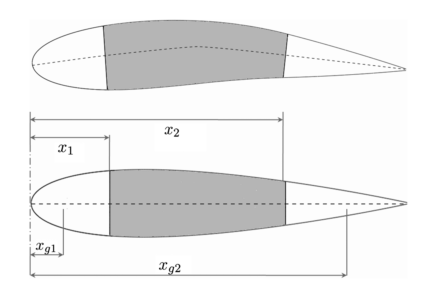
\includegraphics[width=0.8 \textwidth]{state-of-the-art/chiral-sail}
    \caption[Chiral sail concept]{Chiral sail concept. The rib of the airfoil is constituted of a network of chiral unit cells. \cite{Airoldi2012}}\label{fig:chiral-sail}
  \end{figure}  

\clearpage
\section{Bending-Twist shape adaptation by compliant structural designs} \label{sec:bendingTwist_state}
  %Mention-> Falk's work, compare with the actual design proposal (chiral structure): Compliant Chiral Spar Design, 
  %
  % by designing structural components in which instability occurs in a deliberate way. For that purpose, a structural tailoring procedure providing a particular material anisotropy by varying fibre orientation and thickness of the component is introduced.
  % carbon fibre reinforced plastic (CFRP)

  Following a different approach to achieve wing twist morphing compared to those presented in last section, W. Raither proposed in \cite{Raither2013a} a novel concept of adaptive aeroelastic tailoring by means of the wing-box torsional stiffness modification. In order to achieve this, the shear stiffness $G t$ of one of the webs that conform the wing-box beam is modified. This induces the section's shear centre shifting, which provides an additional torsional deformation for a constant load. This concept is later explained in Section \ref{sec:concept_Model} as the same working principle is used for the technology presented in this work.

  Implementation of the proposed principle required for a material that would provide controllable in-plane shear modulus. A possible solution is proposed in \cite{Bergamini2006} and consisted in the use of electro-bonded laminates that vary its bending stiffness by means of electrostatic forces applied different at points of the structure. Another approach is presented in \cite{Raither2012}, and exploits the time-variable lamination in laminate composite shells provided by the temperature dependence of the elastic modulus of polymers in proximity of their glass transition. Therefore, the proposed concept consists on a semi-passive approach since some energy needs to be spent for the activation of the adaptive interfaces. In \cite{Raither2013} the demonstrator shown in Figure \ref{fig:raither-demonstrator} was built to show the viability of this last approach.

  \begin{figure}[!htpb]
    \centering
    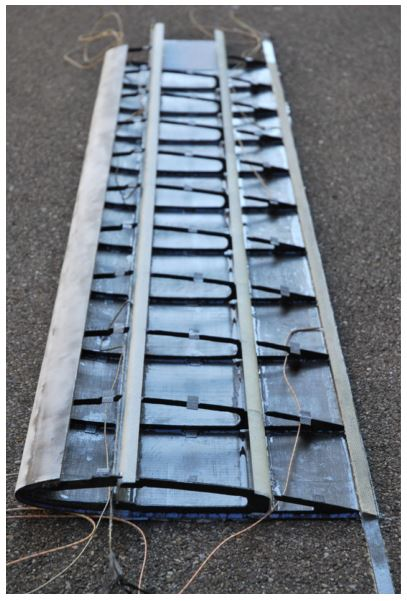
\includegraphics[width=0.6 \textwidth]{state-of-the-art/raither-demonstrator}
    \caption[Inner structure of the experimental wing build to test the concept of adaptive wing-box]{Inner structure of the experimental wing build to test the concept of adaptive wing-box. \cite{Raither2013}}\label{fig:raither-demonstrator}
  \end{figure}

  Finally, in \cite{Runkel2016} the variation of in-plane shear modulus is proposed that can be achieved by inducing elastic instabilities on one of the webs of the wing-box. The component is manufactured with a particular material anisotropy utilizing unidirectional CFRP. The appearance of plate buckling at the root on the specially designed web, as shown in Figure \ref{fig:plate-buckling}, induces the shear centre location shifting and the torsional stiffness of the structure, thus leading to a purely passive bending-twist coupling. In \cite{Andreas2015}, the mechanical response was investigated using FE simulations and experimental testing on a manufactured demonstrator of the concept.

  \begin{figure}[!htpb]
    \centering
    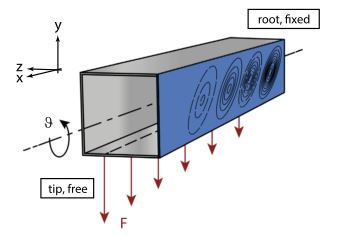
\includegraphics[width=0.7 \textwidth]{state-of-the-art/plate-buckling}
    \caption[Plate bucking on one of the webs of the wing-box beam]{Plate bucking on one of the webs of the wing-box beam. The drawing shows a qualitative view of the buckling field. \cite{Runkel2016}}\label{fig:plate-buckling}
  \end{figure}

\clearpage
\section{Rationale for the thesis} \label{sec:rationale_state}

  This thesis is embed within the current research that it is been carried out at CMAS in seek of wing twist morphing achieved through variable stiffness wing-box structures that acquire this property undergoing elastic instabilities. 

  As shown in the literature review presented in \cite{Hu2015} and \cite{Reis2015}, the use of buckling-induced technologies is a promising technique to achieve the desired behavior in recent developments of smart structures. Traditionally, elastic instabilities were avoided in the structural designs due to the significant loss of load-carrying capacity and large deformations occurring as a consequence of such an event. However, in the scope of the so called motion-related applications of buckling-induced technologies, the capability of small perturbations to generate sudden snapping behavior in elastic elements enables the structure to dynamically change its configuration, being this beneficial for applications such the one considered in the present work. Also, the possibility of minimizing the actuation force required during shape recovery due to the elastic state of the structure becomes interesting.

  In parallel, when it comes to the bending-twist shape adaptation by compliant structural designs, some of the solutions already introduced in this chapter are able to modify the wing-box torsional stiffness for a pre-defined shape variation or are optimized for a given actuation lay-out, whereas the adoption of a structural concept such as a chiral lattice offers a wide range of possibilities in terms of tailoring. In particular, the chiral structures that posses curved ligaments are the design option for the concept proposed in this work. This design of chiral structure was already manufactured and tested in another project completed at CMAS \cite{Vincenz2017}.

  Thereby, for the approach presented in this work, the working principle introduced by \cite{Raither2013a} and explained in Sections \ref{sec:bendingTwist_state} is combined with the special properties of the chiral structures exposed in Section \ref{sec:chiral_state} to conform the proposed principle. 

  In the scope of this thesis, a numerical model model will be built of the whole wing-box assembly. The evolution of the buckling phenomena for in the structure will be characterized and the effect of the different design parameters on the structure pre-buckling and post-buckling response will be assessed. The aim is to provided a suitable computational environment to achieve in-deep understanding of the proposed working principle and assist the manufacture of a future demonstrator.

  It is expected that the proposed technology will be suitable for environments where a rapid shape adaptation is required. Such applications may include to increase the critical speed for load alleviation purposes.